\chapter{Results}\label{chap:results}

\paragraph{}In this thesis, we undertake a thorough investigation of data embeddings and their effectiveness in predicting SSH keys within OpenSSH memory dumps. The results are methodically structured, starting with Data Preprocessing, where we lay a solid foundation by preparing the data for in-depth analysis. We proceed to evaluate Deep Learning Models, analyzing their architecture and limitations. This is succeeded by Feature Engineering, where we meticulously refine our data to improve model accuracy. Through Clustering analysis, we explore and identify underlying patterns within the data. Ultimately, we employ Classification techniques to accurately predict and categorize SSH keys, thus demonstrating the practical implications and utility of our research. 
    

\section{Data Preprocessing}

\paragraph{}In the data preprocessing stage, we meticulously calculated each embedding four times, which included the deep learning models. This repetition was to test all combinations of the two filters—entropy and chunk size. The purpose of this thorough approach was to discern the effectiveness of each filter, both individually and in combination, providing us with a clearer understanding of their impact on the data and the subsequent results. The different datasets used are detailed in Section \ref{sec:annexe:all_dataset}. The dataset codes are explained in the following table~\ref{tab:results:dataset_codes}:

\begin{table}[ht]
    \centering
    \begin{tabular}{|p{0.3\linewidth}|p{0.6\linewidth}|}
    \hline
    Dataset Code & Meaning \\ 
    \hline
    value\_node\_embedding & First graph embedding, with all nodes~\ref{sec:embedding:first_graph} \\ \hline
    chunk\_top\_vn\_semantic\_embedding & First graph embedding, keeping only the first block of each chunk~\ref{sec:embedding:first_graph_only_first_block} \\ \hline
    chunk\_semantic\_embedding & Second graph embedding~\ref{sec:embedding:updated_graph} \\ \hline
    chunk\_statistic\_embedding & Statistical embedding~\ref{sec:embedding:statistical} \\ \hline
    chunk\_start\_bytes\_embedding & Start bytes embedding~\ref{sec:embedding:trim_method} \\ \hline
    chunk\_extraction & Raw byte extraction with filters, to be fed into the deep learning model\\ \hline
    \end{tabular}
    \caption{Meanings of Dataset Codes}
    \label{tab:results:dataset_codes}
\end{table}


\section{Deep Learning Models}

\paragraph{}The exploration of hyperparameters is documented in Section \ref{sec:annexes:deep_learning_hyperparameters}. During our experiments, we encountered instances where some models either ran out of memory, as noted in Sections \ref{sec:annexe:out_of_memory_instances_classifications} and \ref{sec:annexe:out_of_memory_instances_clustering}, or experienced timeouts, detailed in Section \ref{sec:annexe:timeout_instances}. Consequently, our discussion will be confined to the results yielded by the models that successfully completed their runs.

\paragraph{}Within the cohort of operational deep learning models, we endeavored to identify the most proficient instance for each algorithm, whether it was Transformers or Word2Vec. However, we encountered a scarcity of successful instances, which impeded our ability to conclusively determine the optimal hyperparameters or to fully understand their impact on the classification metrics. It was observed that instances with a larger word size and a reduced embedding dimension were more likely to succeed, presumably due to the decreased computational load they required.

\section{Feature Engineering}
\paragraph{}During our feature engineering phase, we encountered a challenge that led to the elimination of certain embeddings. This was due to the invariance observed in the columns, an issue that is elaborated upon in Section \ref{sec:annexe:feature_engineering_fails}. The specific embedding that was rendered ineffective and subsequently removed was the semantic embedding of the first graph, as discussed in Section \ref{sec:embedding:graph_embedding}. This elimination was necessary regardless of whether the filter on the first block of each chunk was applied. The primary shortcoming of this embedding was its inability to generate a sufficient number of ancestors to provide useful information. This inadequacy arose because only a minor segment of the value nodes were being pointed to by pointers, which significantly limited the utility of the embedding. In contrast, the second graph managed to compress the information effectively, thereby validating the semantic embedding by conveying more meaningful data for each node.

\paragraph{}The instances that successfully passed the feature engineering stage are meticulously recorded in Section \ref{sec:annexe:feature_engineering_results}. Here, the eight most significant columns are identified.

\section{Clustering}
\paragraph{}In the clustering phase of our analysis, we categorized the data into distinct groups: label 1 for SSH keys, label 2 for "ssh\_struct", label 4 for "session\_state\_struct", and label 0 for the remainder. The detailed outcomes of this clustering are presented in appendix \ref{sec:annexe:clustering_results}. Our examination revealed that the majority of clusters did not exhibit discernible patterns. However, certain datasets, such as those represented by chunk\_start\_bytes\_embedding (23) in Table \ref{tab:23_single_instance_clustering_results} and chunk\_statistic\_embedding (18) in Table \ref{tab:18_single_instance_clustering_results}, maintained a ratio of labels similar to that of the original dataset.


\paragraph{}Interestingly, the clusters derived from deep learning models typically displayed an even distribution of labels, with approximately one quarter of the data falling into each category. An exception to this trend was observed in the Word2Vec 3 Clustering Results on dataset 25 (with chunk size filter), as shown in Table \ref{tab:25_word2vec_3_clustering_results}, which consisted of three clusters with seemingly random label proportions.

\paragraph{}The results from the clustering analysis were not entirely definitive, indicating that there is substantial room for improvement in the methodology. Future efforts in this area would benefit from a more refined approach to enhance the clarity and significance of the clustering outcomes.

\section{Classification}

\paragraph{}The classification results of our study, detailed in appendix \ref{sec:annexe:classification_results}, yielded highly promising results. The performance of various instances, particularly in terms of accuracy, is depicted in the graphical representation found in Figure \ref{fig:results:best_accuracy_instances}, which ranks the instances from best to worst.

\begin{figure}[ht]
    \centering
    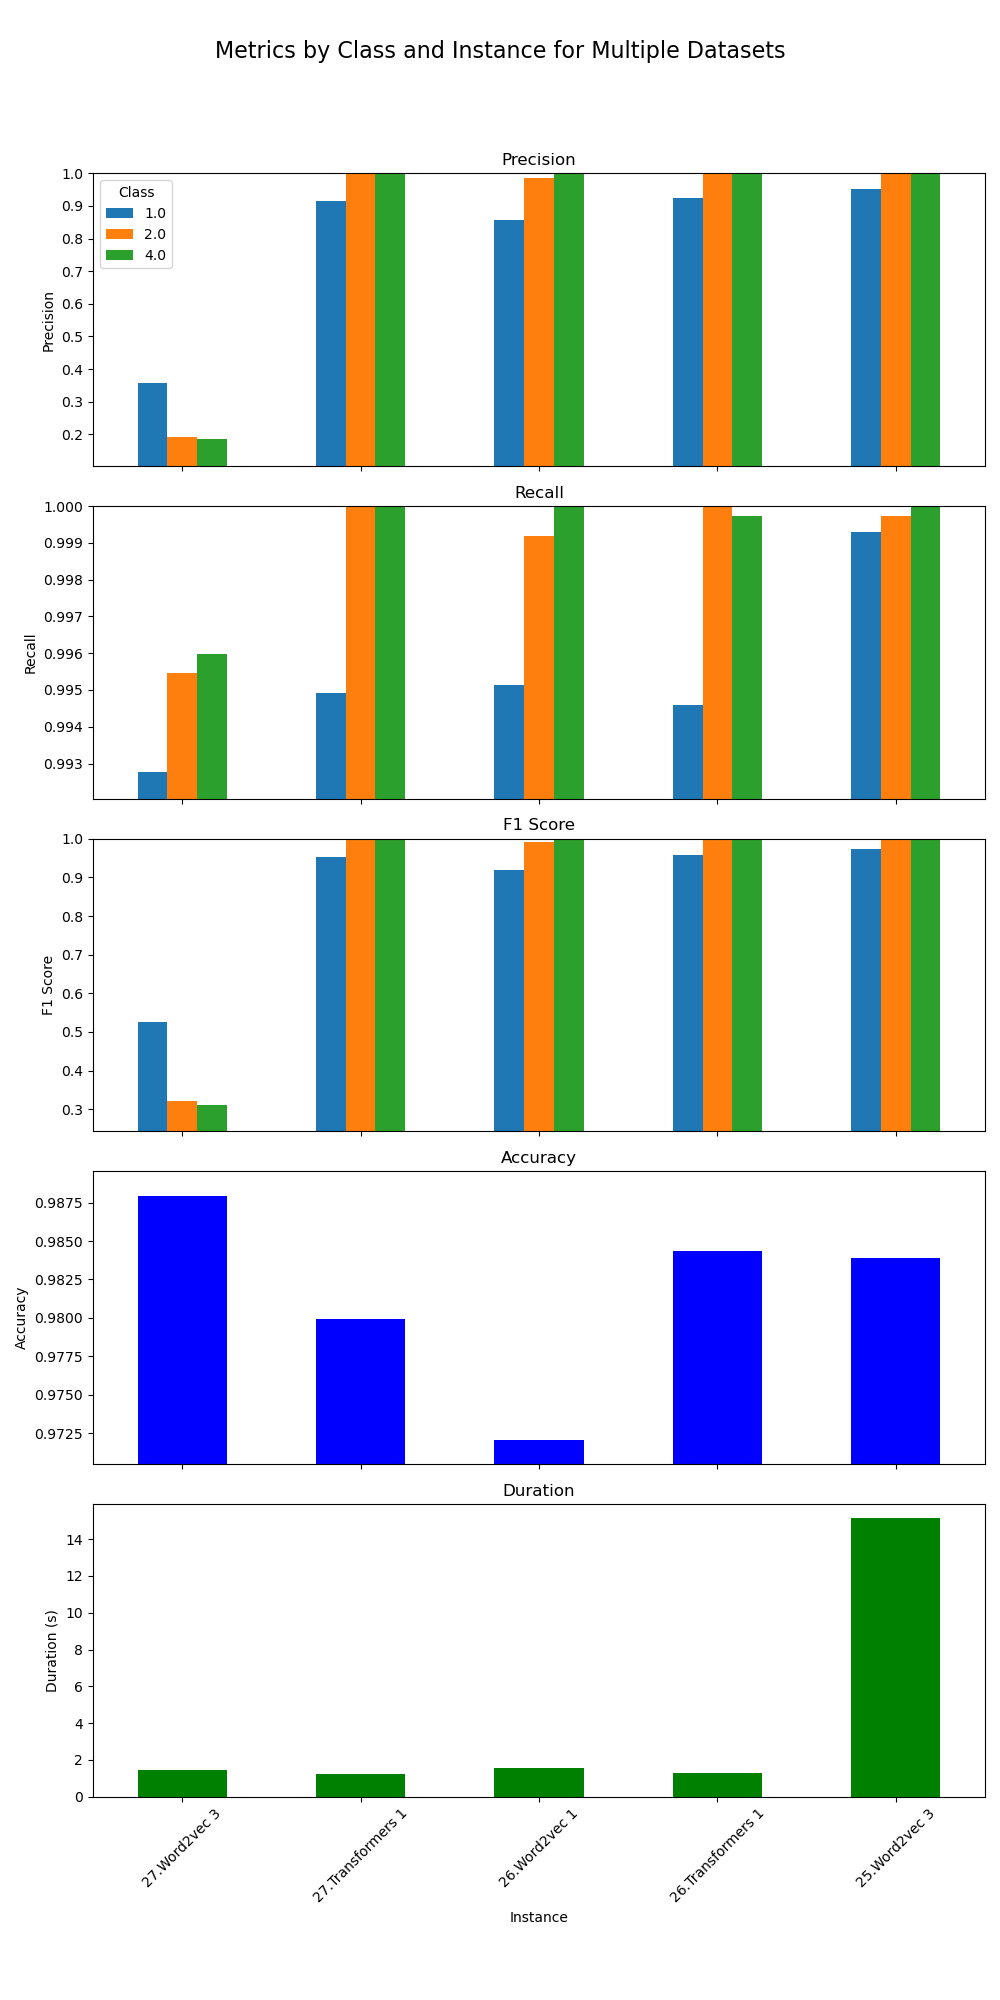
\includegraphics[width=0.6\textwidth]{img/annexes/Best Accuracy (by instances).png}
    \caption{Metrics for the best instances (accuracy)}
    \label{fig:results:best_accuracy_instances}
\end{figure}

\paragraph{}The two top-performing instances, both utilizing chunk\_start\_bytes\_embedding, achieved remarkable accuracy scores of 99.90\% with the chunk size filter~\ref{tab:21_single_instance_classifiers_results} and 99.84\% without the filter~\ref{tab:20_single_instance_classifiers_results}. Following closely was chunk\_semantic\_embedding with the chunk size filter, securing an accuracy of 99.70\%~\ref{tab:9_single_instance_classifiers_results}. Notably, the first deep learning model to make an appearance in the ranking was a Word2Vec model, which, with both entropy and chunk size filters applied, attained an accuracy of 98.79\%, placing it sixth overall~\ref{tab:27_word2vec_3_classifiers_results}.

\paragraph{}When focusing on recall for label 1, the best instance was chunk\_start\_bytes\_embedding without any filter, achieving a perfect recall of 100\%~\ref{tab:20_single_instance_classifiers_results}, as shown in Figure \ref{fig:results:best_label_1_recall_instances}. The second-best was again chunk\_start\_bytes\_embedding, this time with both entropy and chunk size filters, achieving a recall of 99.99553\%~\ref{tab:23_single_instance_classifiers_results}. The first deep learning model, a Word2Vec instance with both filters, ranked third with a recall of 99.95\%.

\begin{figure}[ht]
    \centering
    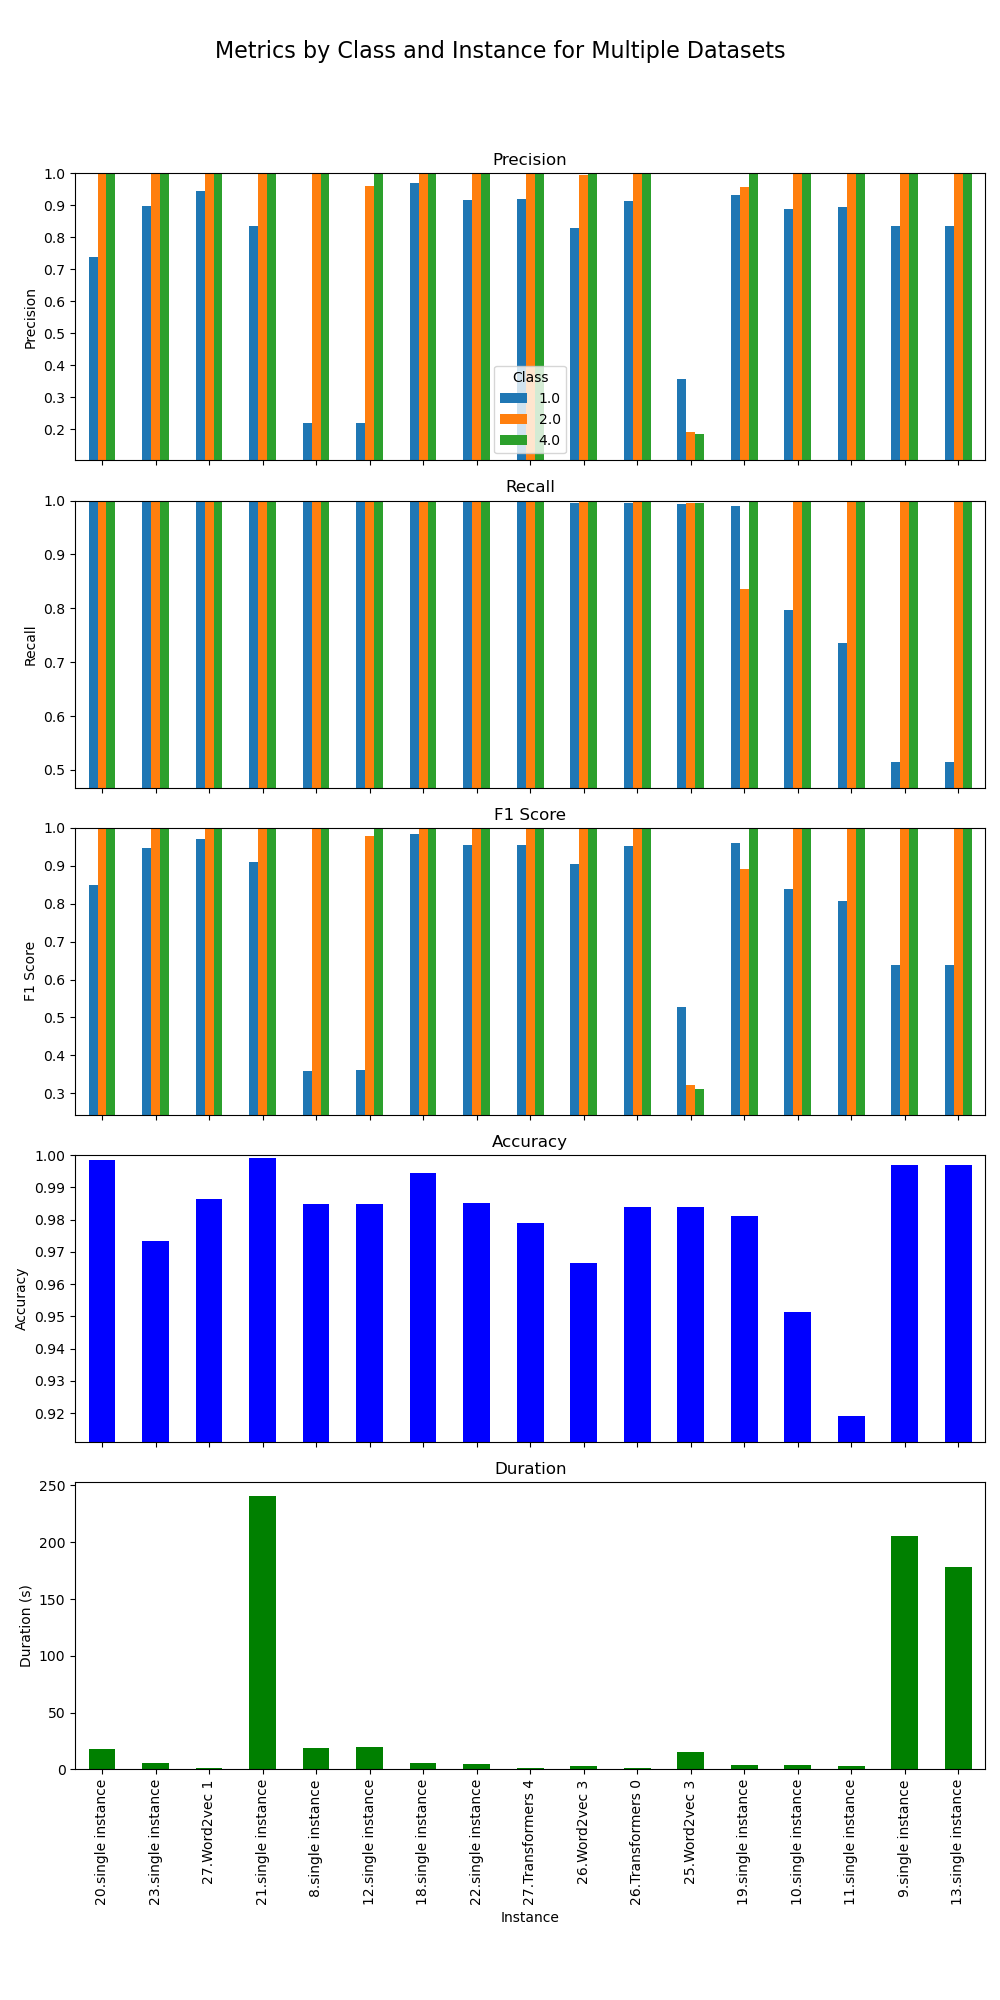
\includegraphics[width=0.6\textwidth]{img/annexes/Best 1.0 Recall (by instances).png}
    \caption{Metrics for the best instances (Label 1 recall)}
    \label{fig:results:best_label_1_recall_instances}
\end{figure}

\paragraph{}As for precision on label 1, the highest achievement was recorded by chunk\_statistic\_embedding with the entropy filter, which reached a precision of 96.86\%~\ref{tab:18_single_instance_classifiers_results}, as illustrated in Figure \ref{fig:results:best_label_1_precision_instances}. The second-highest precision came from a Word2Vec deep learning model with both entropy and chunk size filters, scoring 95.19\%.

\begin{figure}[ht]
    \centering
    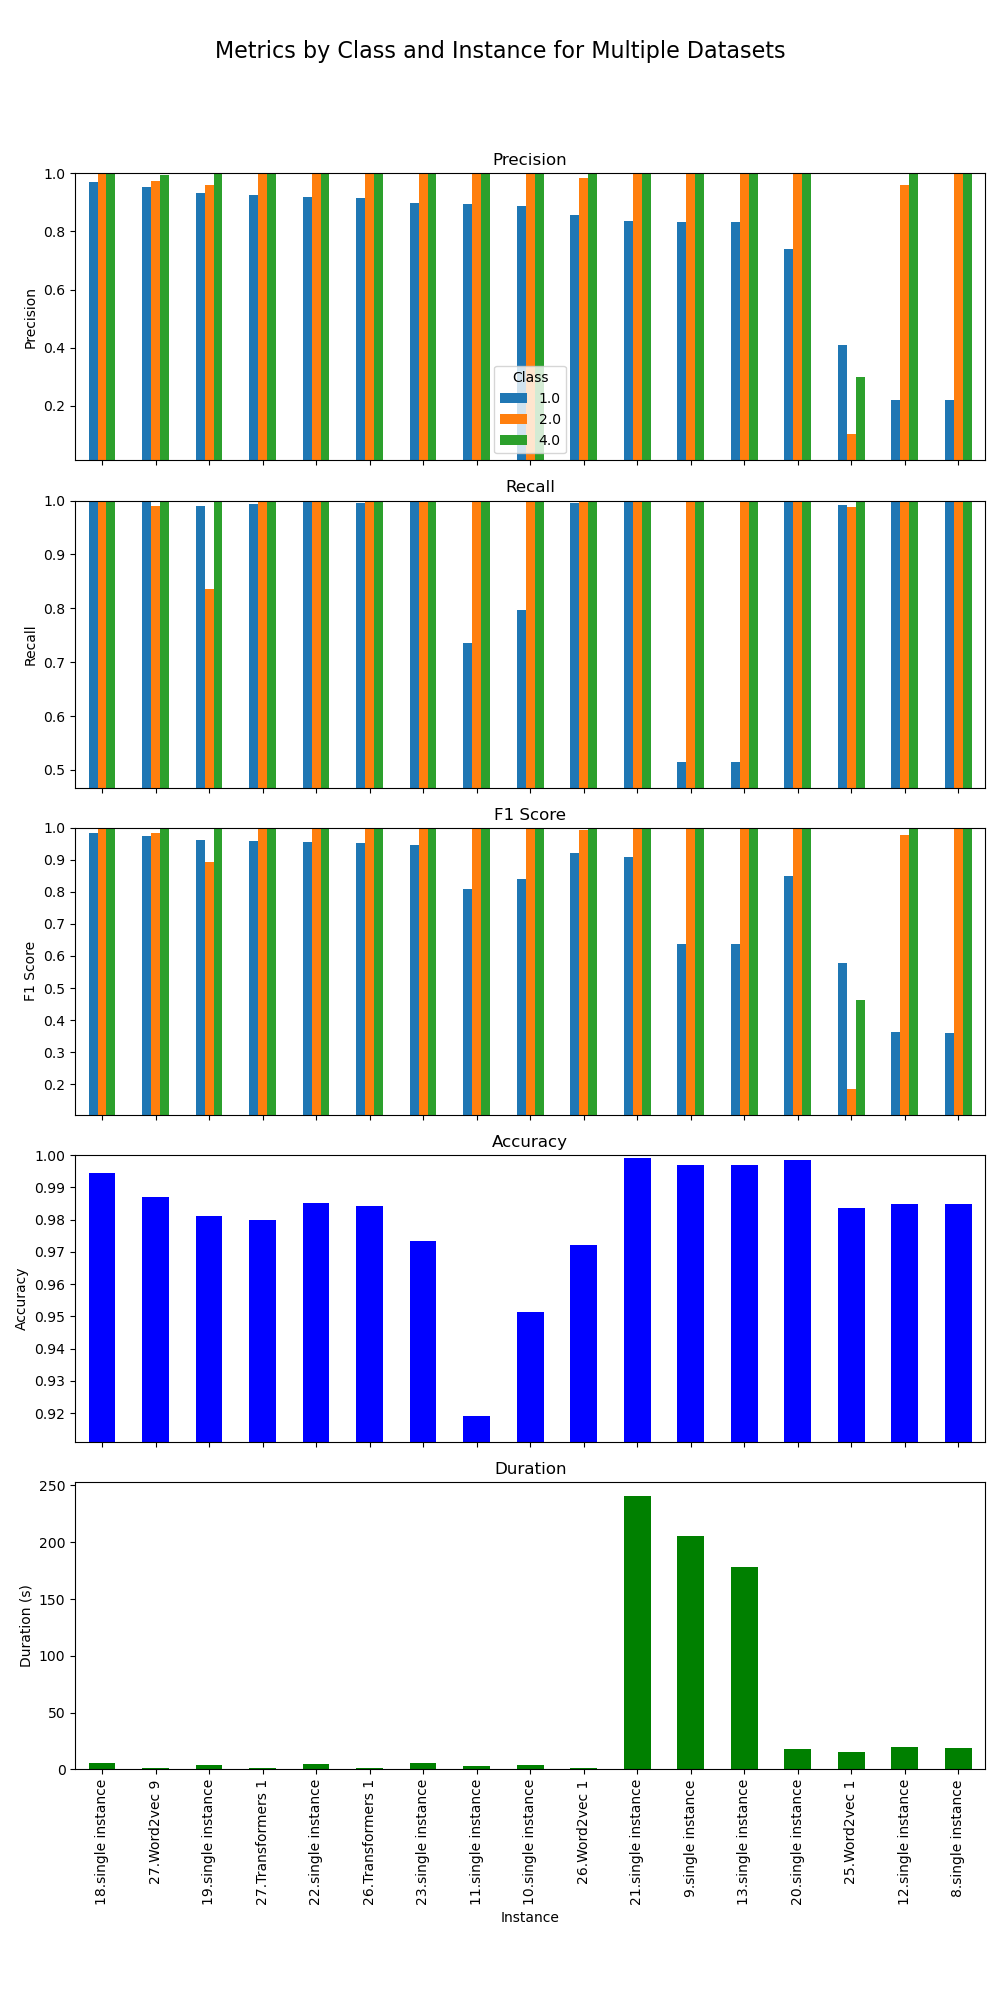
\includegraphics[width=0.6\textwidth]{img/annexes/Best 1.0 Precision (by instances).png}
    \caption{Metrics for the best instances (Label 1 precision)}
    \label{fig:results:best_label_1_precision_instances}
\end{figure}

